\chapter{Cas d'utilisation}

\section{Schéma}

\begin{figure}
  \centering
  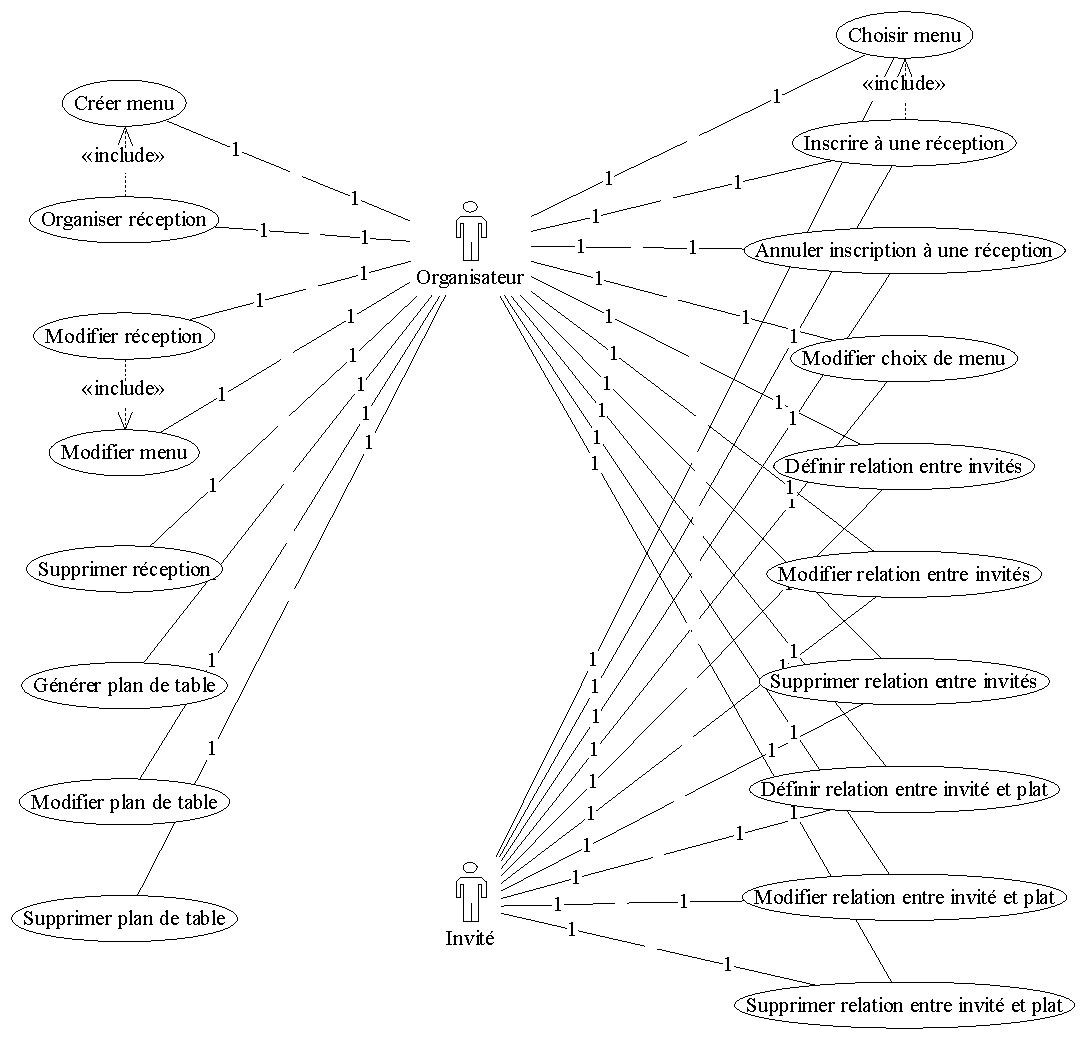
\includegraphics[scale=.88]{IMG/use_cases}
  \caption{Cas d'utilisation}
  \label{img_use_cases}
\end{figure}

L'image \refpage{img_use_cases} représente les cas d'utilisation de l'application. Les cas qui seront développés ici sont \og{}Générer plan de table\fg{}, \og{}Inscrire à une réception\fg{} et \og{}Définir relation entre invités\fg{}

\section{Scénarios}

\subsection{Générer plan de table}

\begin{figure}
  \centering
  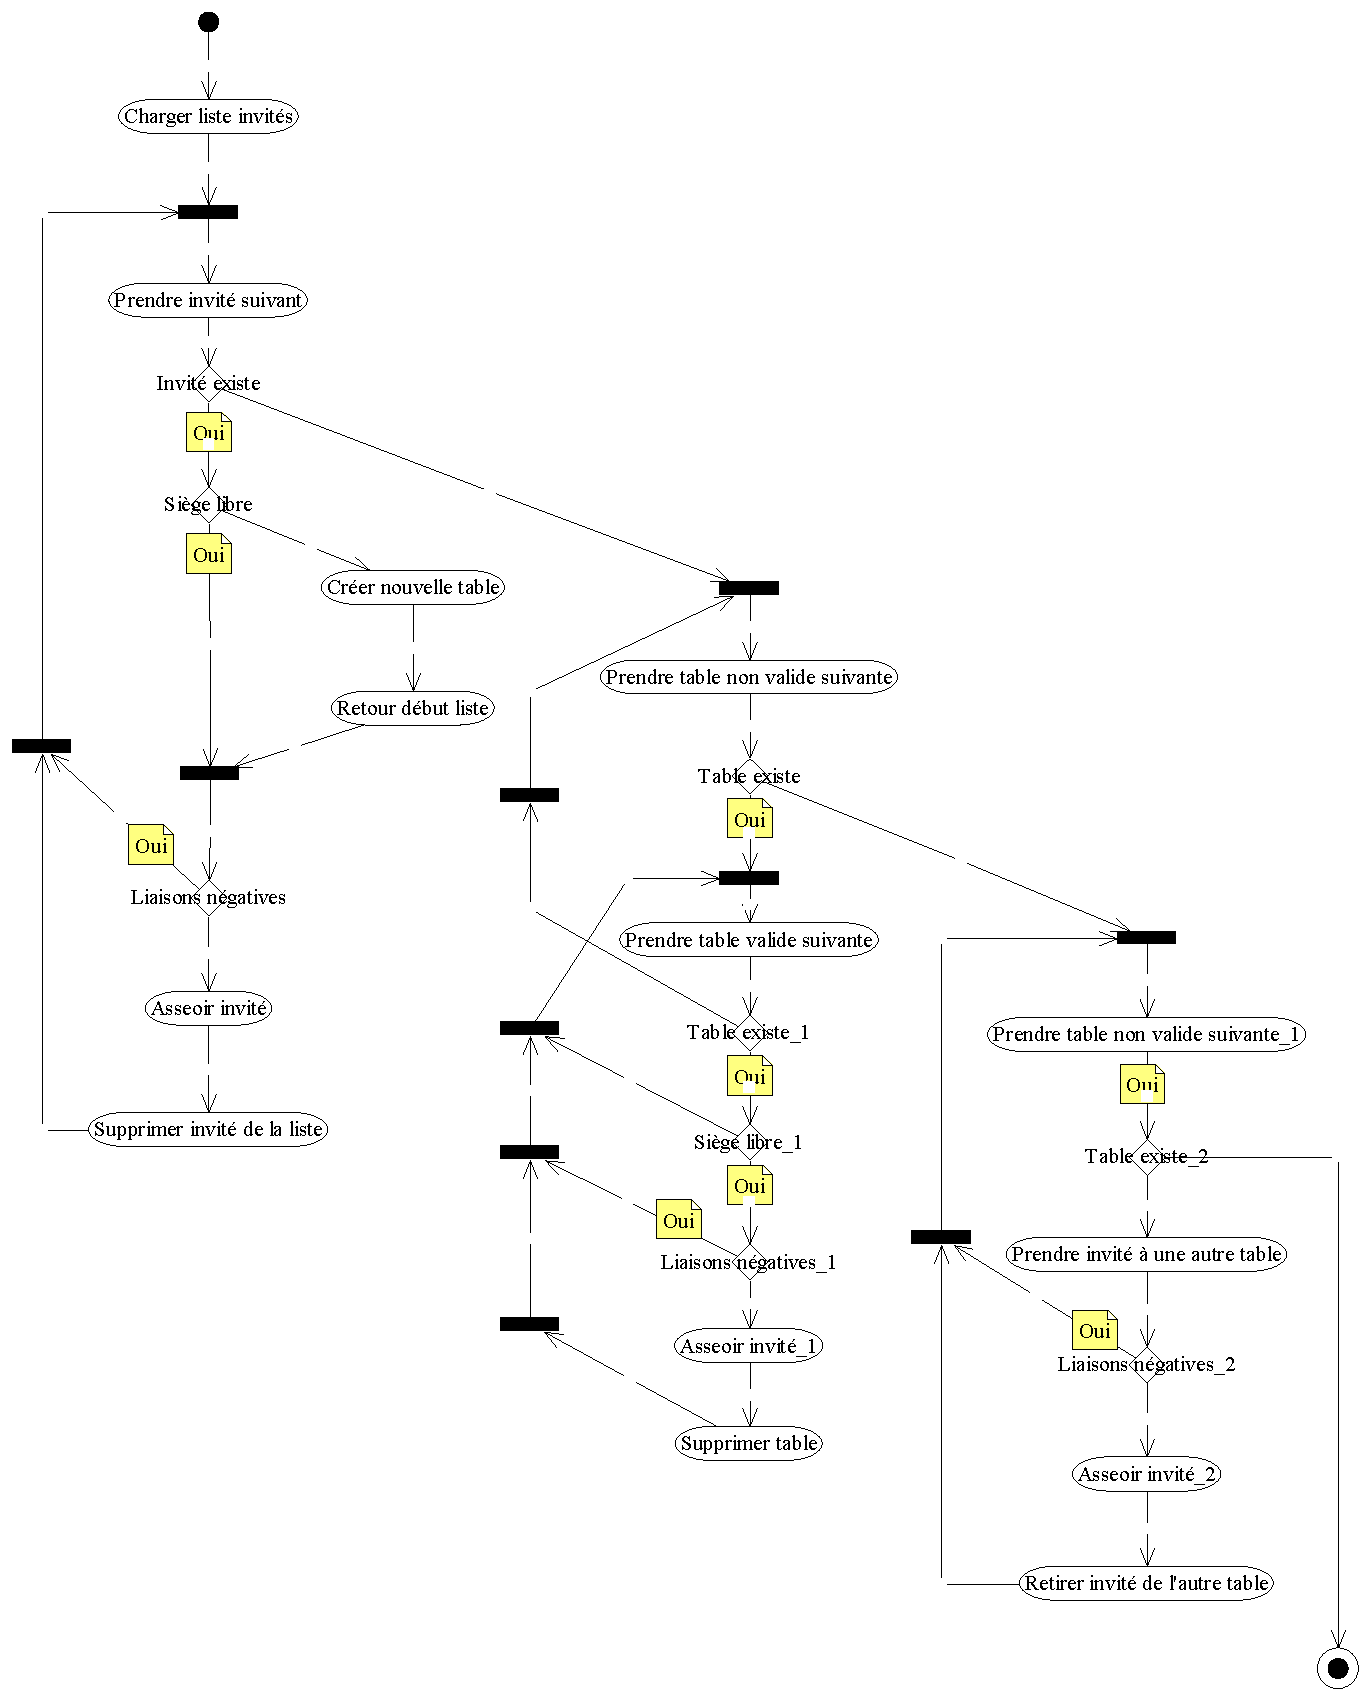
\includegraphics[width=\textwidth]{IMG/da_plan_tables}
  \caption{Diagramme d'activité -- génération du plan de table}
  \label{img_da_plan_tables}
\end{figure}

Pour générer le plan de table d'une réception, nous allons parcourir la liste des invités inscrits à cette réception. Nous allons prendre le premier invité et l'asseoir à une table. Ensuite, nous prenons l'invité suivant. S'il n'y a aucune relation négative entre ce dernier est les invités déjà assis, nous le plaçons à la table et le retirons de la liste des personnes à placer.

Lorsque toutes les places d'une tables seront occupées, nous passerons à la table suivante et reprenons au début de la liste des personnes à placer.

Une fois que nous aurons placé toutes les personnes, nous veillerons à ce qu'aucune table ne contienne qu'une seule personne. Pour ce faire, nous allons prendre chaque invité assis seul et tenter de l'asseoir à une table qui n'est pas complète. Si après cela, il reste encore des invités qui sont seuls à une table, nous prendrons des invités à d'autres tables pour les assoir avec eux.

La figure \refpage{img_da_plan_tables} illustre le diagramme de séquence de ce scénario.

\subsection{Inscrire à une réception}

\begin{figure}
  \centering
  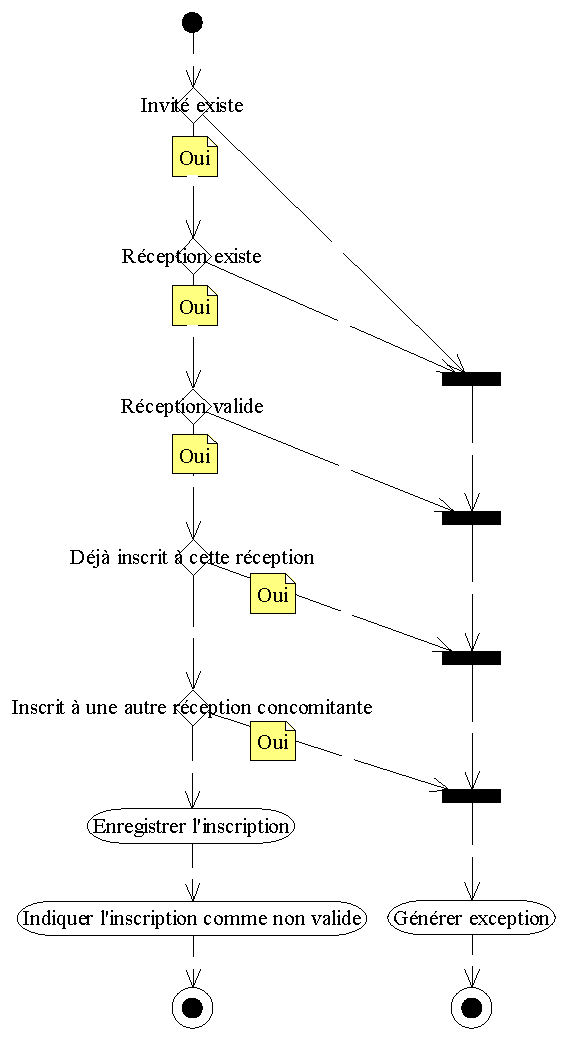
\includegraphics[scale=.88]{IMG/da_inscription_reception}
  \caption{Diagramme d'activité -- inscription à une réception}
  \label{img_da_inscription_reception}
\end{figure}

Avant de pouvoir inscrire un invité à une réception, nous allons vérifier si elle est valide, c'est à dire s'il y a un menu présent composé de tous les types de plat. Ensuite, nous vérifions si l'invité n'est pas déjà inscrit à cette réception et s'il n'est pas déjà inscrit à une autre réception qui se passe en même temps.

Si tous les tests sont concluants, l'inscription sera enregistrée. Elle ne sera toutefois validée que lorsque l'invité aura choisi ses plats pour cette réception.

La figure \refpage{img_da_inscription_reception} illustre le diagramme de séquence de ce scénario.

\subsection{Définir relation entre invités}

\begin{figure}
  \centering
  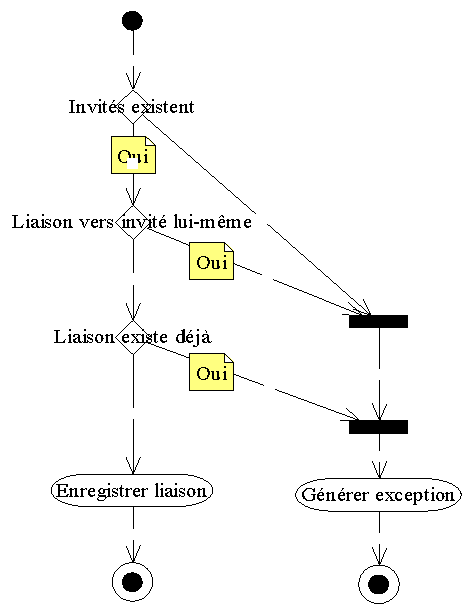
\includegraphics[scale=.88]{IMG/da_definir_relation_entre_invites}
  \caption{Diagramme d'activité -- définir une relation entre invités}
  \label{img_da_definir_relation_entre_invites}
\end{figure}

Avant d'enregistrer une relation entre invités, nous allons d'abord vérifier que l'invité n'essaie pas d'établir une relation ave lui-même. Aussi, nous allons vérifier si la relation n'existe pas déjà.

Si tous les tests sont concluants, la relation sera enregistrée.

La figure \refpage{img_da_definir_relation_entre_invites} illustre le diagramme de séquence de ce scénario.
